\documentclass[10pt,conference,compsocconf]{IEEEtran}

%\usepackage{times}
%\usepackage{balance}
\usepackage{url, amsmath, amssymb}
\usepackage{graphicx}    % For figure environment

\newcommand{\spacing}{\hspace{1cm}}
\begin{document}
    \title{Collaborative Filtering}

    \author{
    Filip Batur\spacing Patrik Okanovic\spacing Rafael Sterzinger\spacing Fatjon Zogaj\\
    ETH Zurich, Switzerland
    }

    \maketitle

    \begin{abstract}

    \end{abstract}


    \section{Introduction}


    \section{Related Work}


    \section{Models and Methods}

    \subsection{Singular Value Decomposition}

    \subsection{Non-Negative Matrix Factorization}
    
    \subsection{K-Means Clustering}
    
    In order to provide additional information for models we implement clustering and that way simulate the information about movie categories as in the MovieLens Dataset TODO: CITE. First we initialize the matrix using FM:TODO. Afterwards, we perform Singular Value Decomposition with the rank that showed best results (TODO ref the plot). We get the embeddings using the following expression: assuming $A=U\Sigma V^T$ then embeddings matrix is equal to $\Sigma _k ^{\frac{1}{2}} V_k ^T$. Finally, after obtaining the k-rank movie embeddings we search for the optimal number of clusters in K-Means clustering. We visualize the clusters in 2 dimensions. Since, visualizing in two dimensions does not easily distinct the optimal number of clusters we choose 18 as in the MovieLens dataset as the number of clusters. Picture \ref{movie_category_distribution} shows two peaks in movie categories while other categories look uniformly distributed.
    
    \begin{figure}\label{movie_category_distribution}
        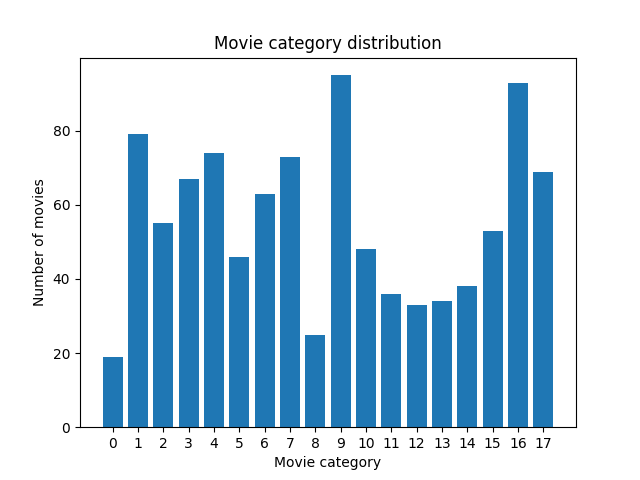
\includegraphics[width=\columnwidth]{figures/movie_category_distribution.png}
        \caption{Distribution of movie categories between 18 categories as in MovieLens dataset.}
    \end{figure}


    \subsection{Autoencoder}
    An autoencoder is a neural network that is trained to attempt to copy its input to its output. 
    Internally, it has a hidden layer $\textbf{h} \in \mathbb{R}^k$ that describes a code used to represent the input.
    The network may be viewed as consisting of two parts: an encoder function $f: \mathbb{R} ^d \rightarrow \mathbb{R} ^k$ and a decoder that produces a reconstruction $g: \mathbb{R} ^k \rightarrow \mathbb{R} ^d$ \cite{Goodfellow-et-al-2016}. Autoencoders have proven to achieve good results in collaborative filtering \cite{inproceedings}. We examine the user-based autoencoder as opposed to item-based autoencoder which achieved a good score in \cite{inproceedings}. Both encoder and decoder consist of feedforward neural networks with ReLU activation functions. We train the model by minimizing the squared reconstruction loss. Important part of the implementation is the fact that inputs are partially observed and therefore we only update those weights that are associated with observed inputs during backpropagation. 
    We found that when both encoder and decoder consist of one layer increasing the encoded dimension up to 500 makes the score better. Furthermore, we have examined the effect of compositionality. Using only two layers in encoder and decoder already performs better than any single layer autoencoder. 
    
    \subsection{Neural Collaborative Filtering}
    Neural Collaborative Filtering approach as proposed by He et al. \cite{DBLP:journals/corr/abs-1708-05031}, tries to jointly learn user-item latent representations as well as the prediction depending on the interactions between different users and items. The network's inputs are indices of users and items. Firstly, an embedding layer maps each user and aeach item to its corresponding latent vector representation. Output of the embedding layers is then concatenated and passed on through fully connected feedforward layers with ReLU activation functions. Finally, output of the network represents the rating associated with the inputted user and item. Network is trained minimizing the mean squared error loss between the predicted and target rating. TODO: erase? Further, improvements would be implementing the network as a classification task between the movie rating rather then regressing the predicted rating.

    \subsection{Kernel Net}

    \subsection{Factorization Machines}

    \subsubsection{User Features}
    \cite{lee_improving_2017}


    \subsubsection{Movie Features}

    \subsection{Ensembles}


    \section{Results and Discussion}

    \subsection{Comparison to Baselines}

    You compare your novel algorithm to \emph{at least two baseline
    algorithms}. For the baselines, you can use the implementations you
    developed as part of the programming assignments.


    \section{Conclusion}

    Organize the results section based on the sequence of table and
    figures you include. Prepare the tables and figures as soon as all
    the data are analyzed and arrange them in the sequence that best
    presents your findings in a logical way. A good strategy is to note,
    on a draft of each table or figure, the one or two key results you
    want to address in the text portion of the results.
    The information from the figures is
    summarized in Table.\cite{anderson04}




    \bibliographystyle{IEEEtran}
    \bibliography{bibliography}
\end{document}
